\section{Diskussion}
\label{sec:Diskussion}

% theoretische werte µ: 69.351 für blei, 50.544 für zink

Die theoretisch ermittelten Werte für die Compton-Absorptionskoeffizienten
\begin{eqnarray}
  \mu_{Pb} &=&   \pm  \,  \mathrm{m^-1} \nonumber \\
  \mu_{Zn} &=&   \pm  \,  \mathrm{m^-1} \nonumber 
\end{eqnarray}
lassen sich mit den experimentiell bestimmten 
\begin{eqnarray}
  \mu_{Pb} &=&   \pm  \,  \mathrm{m^-1} \nonumber \\
  \mu_{Zn} &=&   \pm  \,  \mathrm{m^-1} \nonumber 
\end{eqnarray}
vergleichen. Die Werte aus dem Experiment zeigen eine Abweichung von
\begin{eqnarray}
  \eta_{Pb} &=&   \pm  \,  \mathrm{m^-1} \nonumber \\
  \eta_{Zn} &=&   \pm  \,  \mathrm{m^-1}. \nonumber 
\end{eqnarray}



\section{Anhang}
\label{sec:anhang}

\begin{figure}[H]
  \centering
  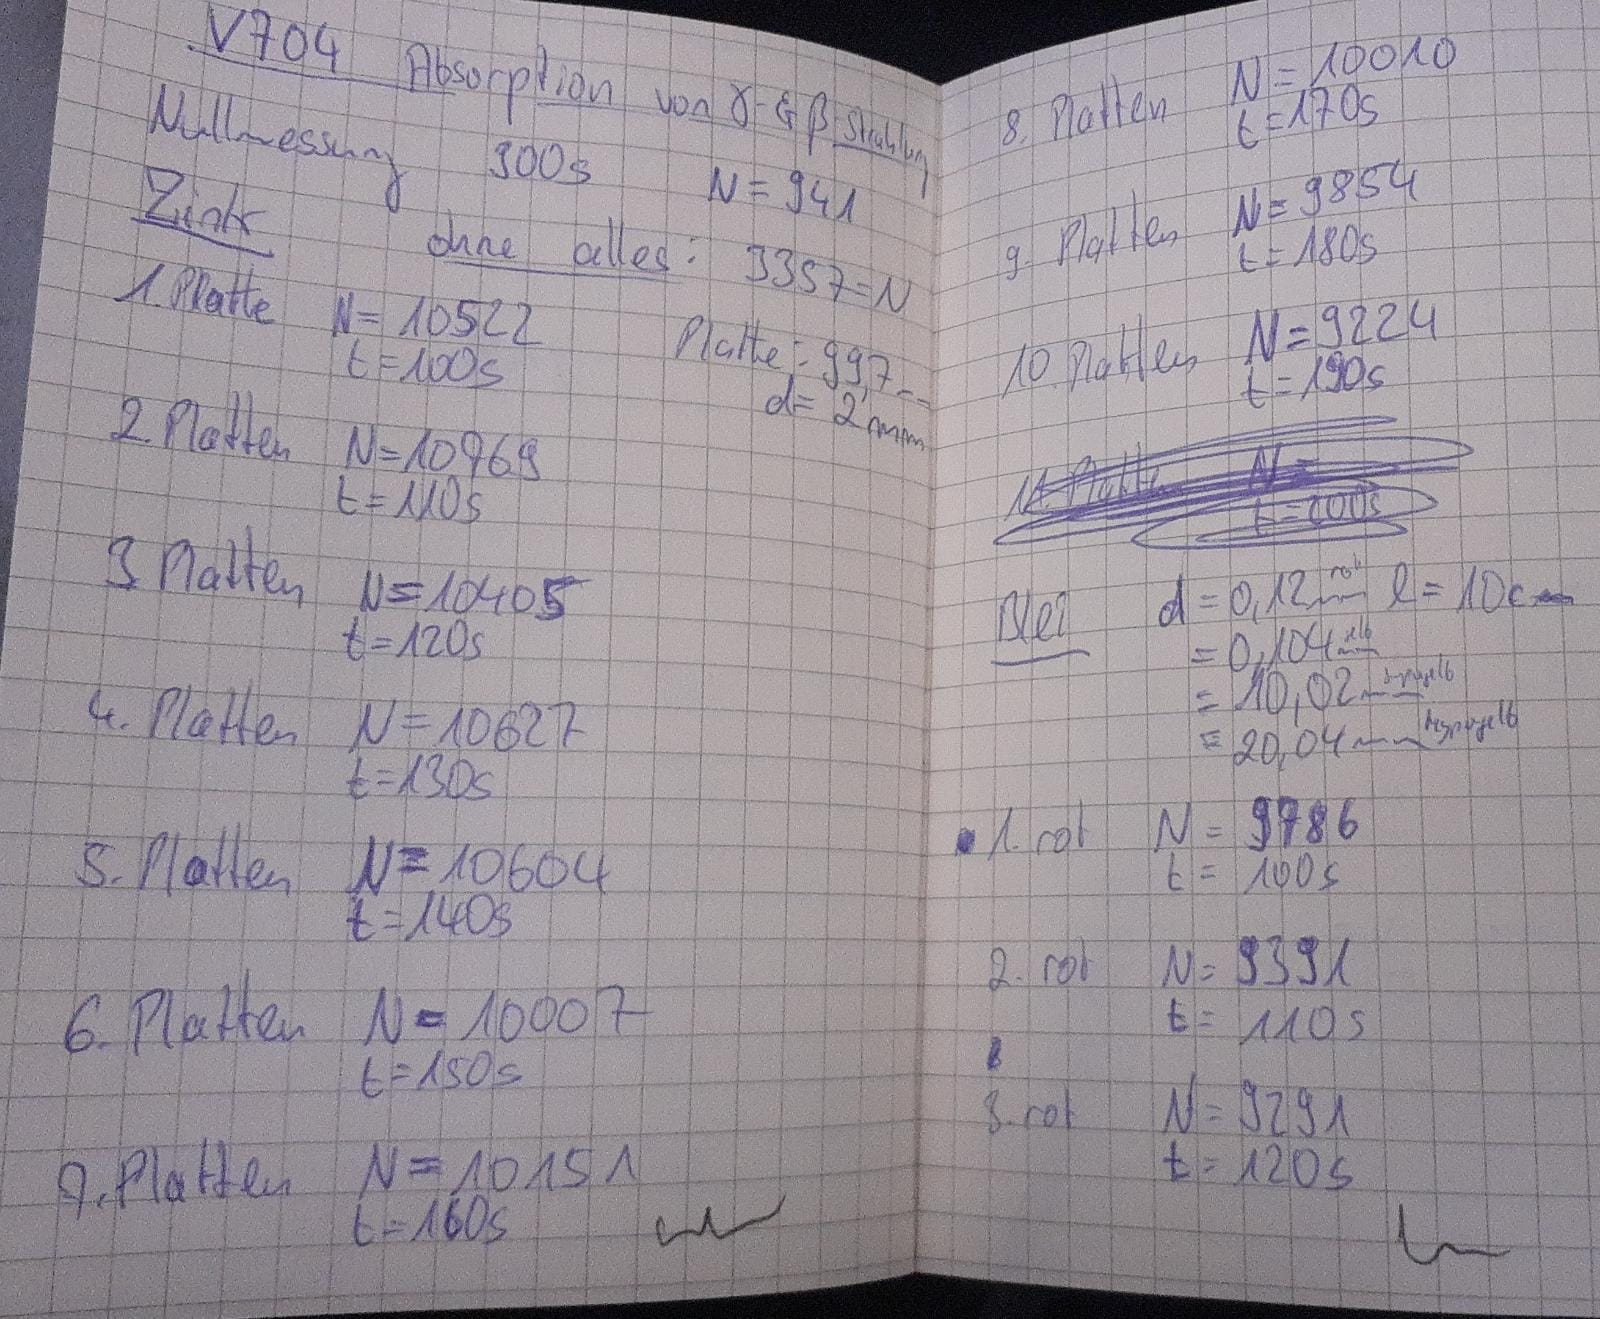
\includegraphics{content/mess1.jpg}
  \caption{Die aufgenommenen Messwerte.}
  \label{fig:mess1}
\end{figure}
\begin{figure}[H]
  \centering
  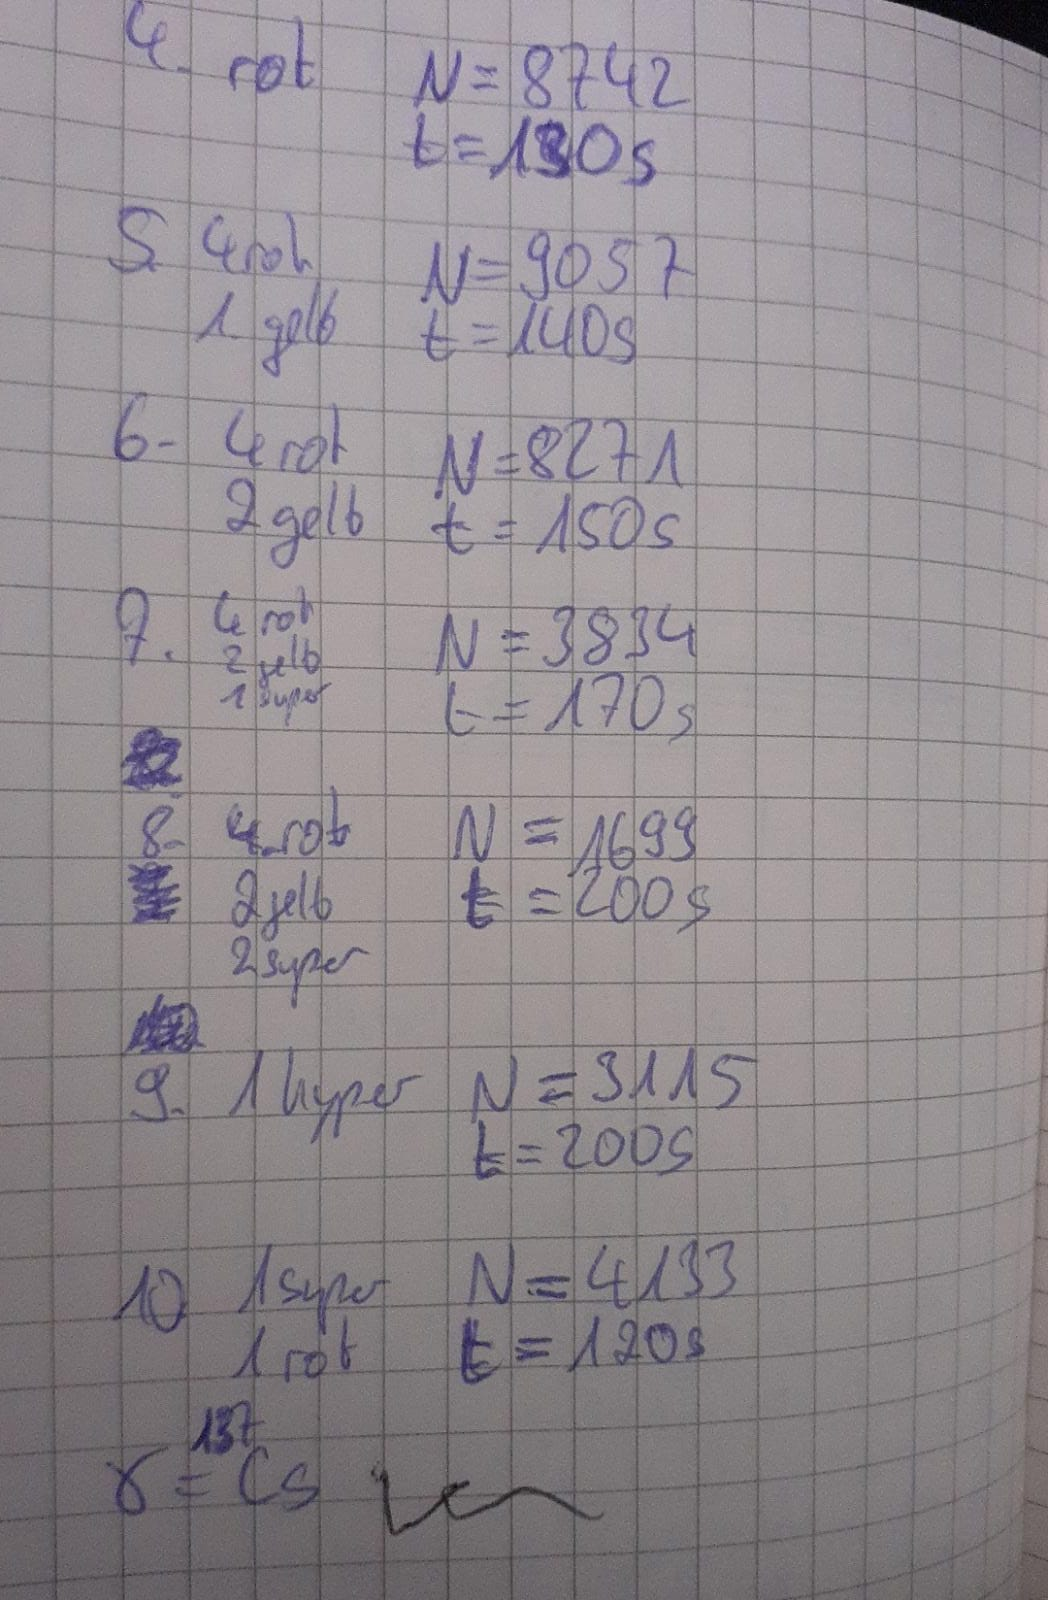
\includegraphics{content/mess2.jpg}
  \caption{Die aufgenommenen Messwerte.}
  \label{fig:mess2}
\end{figure}
\begin{figure}[H]
  \centering
  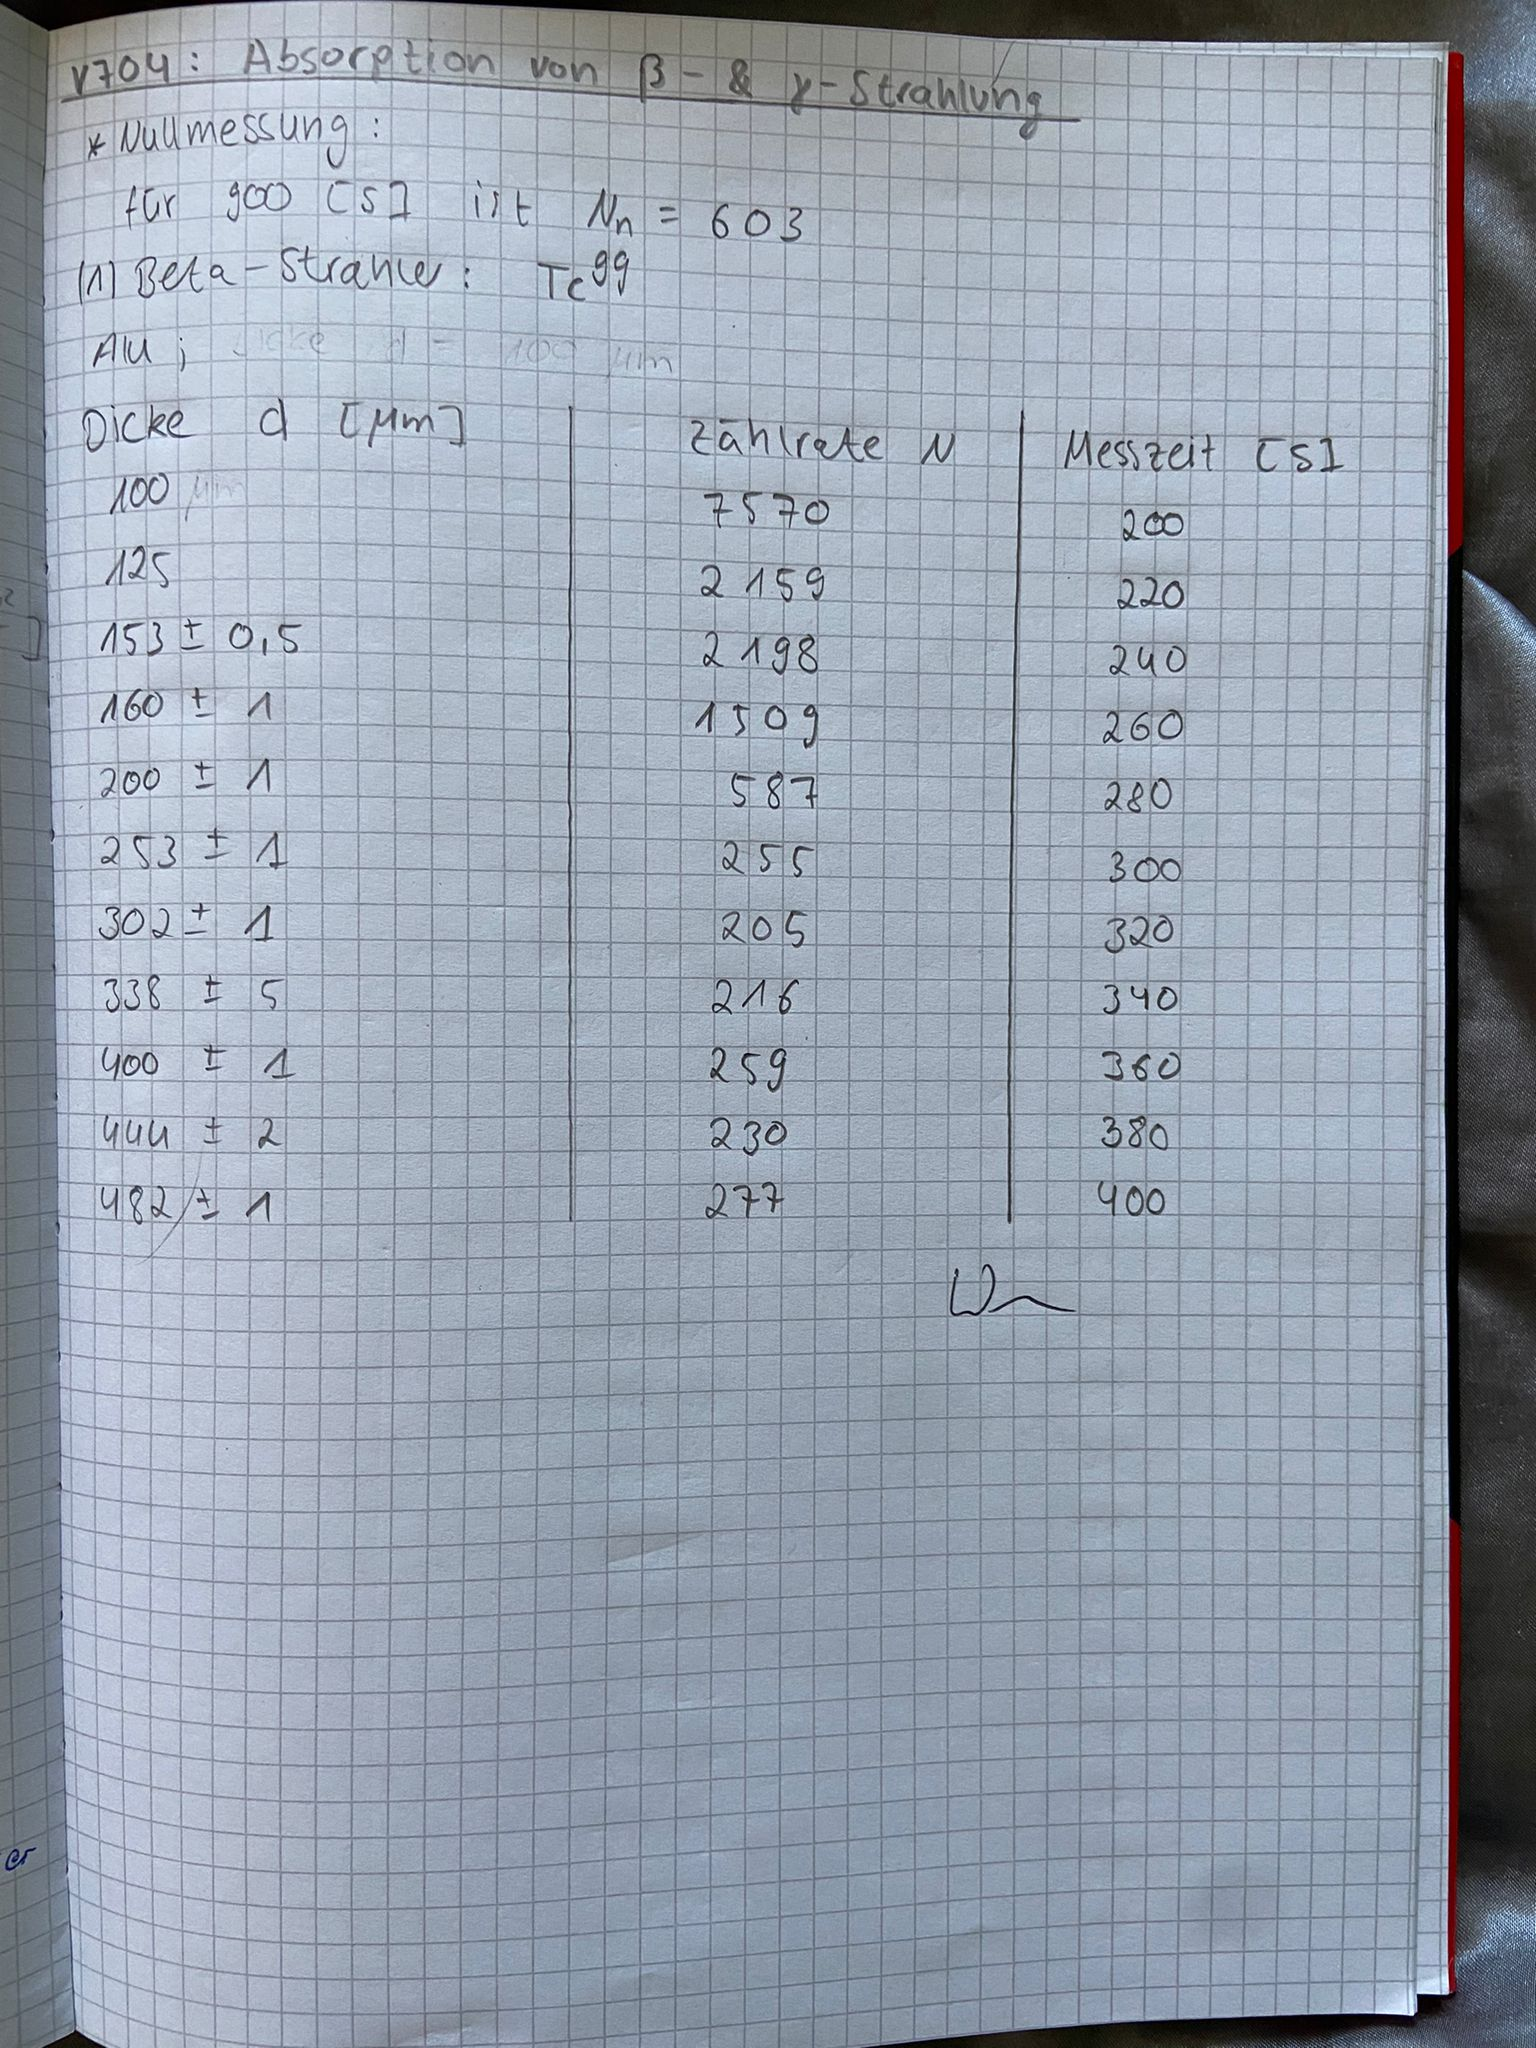
\includegraphics{content/messbeta.jpeg}
  \caption{Die aufgenommenen Messwerte.}
  \label{fig:messbeta}
\end{figure}